\setLTR
$a: 0xAC620014$

$b: 0x0082082A$
\setRTL

\subsubsection*{الف}
در این باید کد اسمبلی معادل با هر دستور را بنویسیم. برای این کار ابتدا اعداد را به باینری تبدیل می‌کنیم:
\setLTR

$a=(10101100011000100000000000010100)_2$

$b=(00000000100000100000100000101010)_2$

\setRTL

حال از این تصویر استفاده کرده و دستورات را شناسایی می‌کنیم:

\setLTR
\qquad\qquad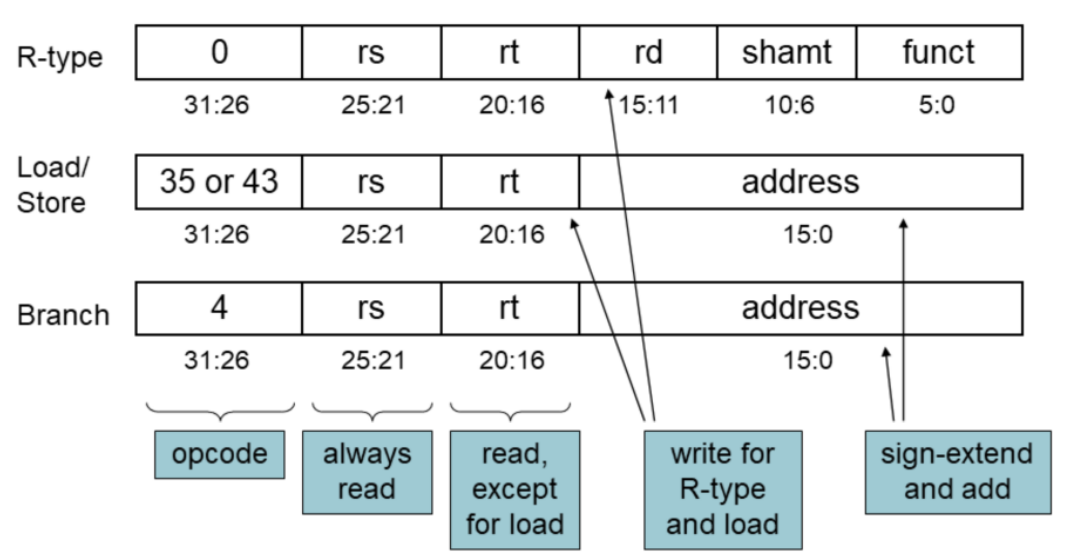
\includegraphics[scale=0.5]{figs/1.png}

$opcode_a = a[31:26] = (101011)_2 = (43)_{10} \longrightarrow store$

$
\begin{cases}
	r_s = a[25:21] = (00011)_2 = (3)_{10} \longrightarrow v_1 \\ 
	r_t = a[20:16] = (00010)_2 = (2)_{10} \longrightarrow v_0 \\
	immediate = a[15:0] = (0000000000010100)_2 = (20)_{10}
\end{cases}\longrightarrow
sw \ \ \$v_0 , 20(\$v_1)
$\\ \\ \\

$opcode_b = b[31:26] = (000000)_2 = (0)_{10} \longrightarrow R-Type$

$
\begin{cases}
	r_s = b[25:21] = (00100)_2 = (4)_{10} \longrightarrow a_0 \\ 
	r_t = b[20:16] = (00010)_2 = (2)_{10} \longrightarrow v_0 \\
	r_d = b[15:11] = (00001)_2 = (1)_{10} \longrightarrow a_t \\
	function = b[5:0] = (101010)_2 \longrightarrow set \ on \ less \ than 
\end{cases} \qquad \longrightarrow
slt \ \ \$a_t \ ,\ \$a_0 \ , \ \$v_0
$\\ \\ \\
\setRTL

\subsubsection*{ب}
خروجی extend sign دستور a ، 16 بیت اول دستور را به یک عدد 32 بیتی تبدیل می‌کند با حفظ علامت:
\setLTR

$output=(00000000000000000000000000010100)_2 = (14)_{16}$

\setRTL

خروجی واحد left shift که توسط دستور b اجرای می‌شود، خروجی واحد extend sign را می‌گیرد و 2 بیت به چپ شیفت می‌دهد.
\setLTR

$output = (010000010000010000010101000)_2 = (20820A8)_{16}$

\setRTL

\subsubsection*{ج}

در این بخش باید مقادیر واحد کنترل ALU را به ازای هر دستور محسابه کنیم. از تصویر زیر کمک می‌گیریم:

\setLTR
\qquad\qquad\qquad\qquad\qquad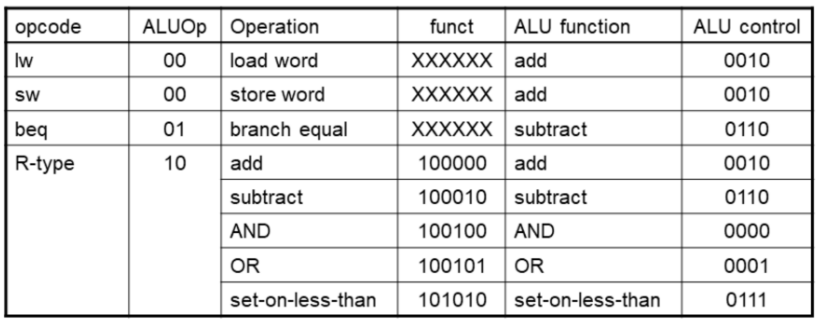
\includegraphics[scale=0.45]{figs/2.png}

$
a\rightarrow lw \rightarrow \begin{cases}
	ALUOp = 00 \\
	funct =  a[5:0] = \times
\end{cases}
$

$
b\rightarrow R Type \rightarrow \begin{cases}
	ALUOp = 10 \\
	funct = b[5:0] = 101010
\end{cases}
$

\setRTL

\subsubsection*{د}

با توجه به این‌که هیچ کدام از دستورات مربوط به دستورات jump و یا branch نیستند، پس در هر دو حالت مقدار برابر است با:

\setLTR

$PC \leftarrow PC + 4$

\setRTL

در شکل زیر مسیرهایی که از آن‌ها این مقادیر به‌دست می‌آیند را می‌بینید:

\setLTR
\qquad\qquad\qquad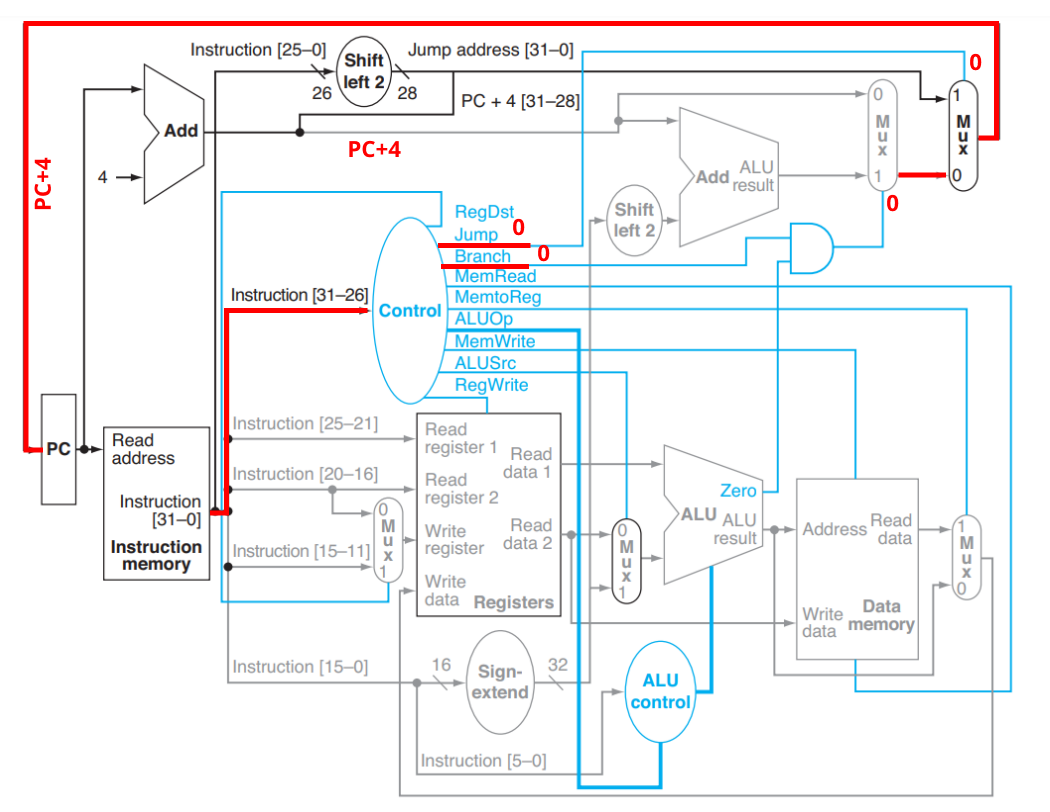
\includegraphics[scale=0.29]{figs/3.png}

\setRTL

\pagebreak


مقدار موجود در هر یک از ثبات‌ها به شرح زیر است:

\setLTR

$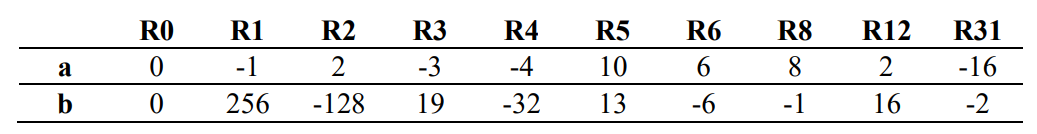
\includegraphics[width=0.7\linewidth]{figs/4}$

\setRTL

\subsection*{ه}

در این بخش باید مقادیر خروجی هر یک از MUX ها را مشخص کنیم. ابتدا به سراغ دستور a می‌رویم:

\setLTR

$\qquad\qquad\qquad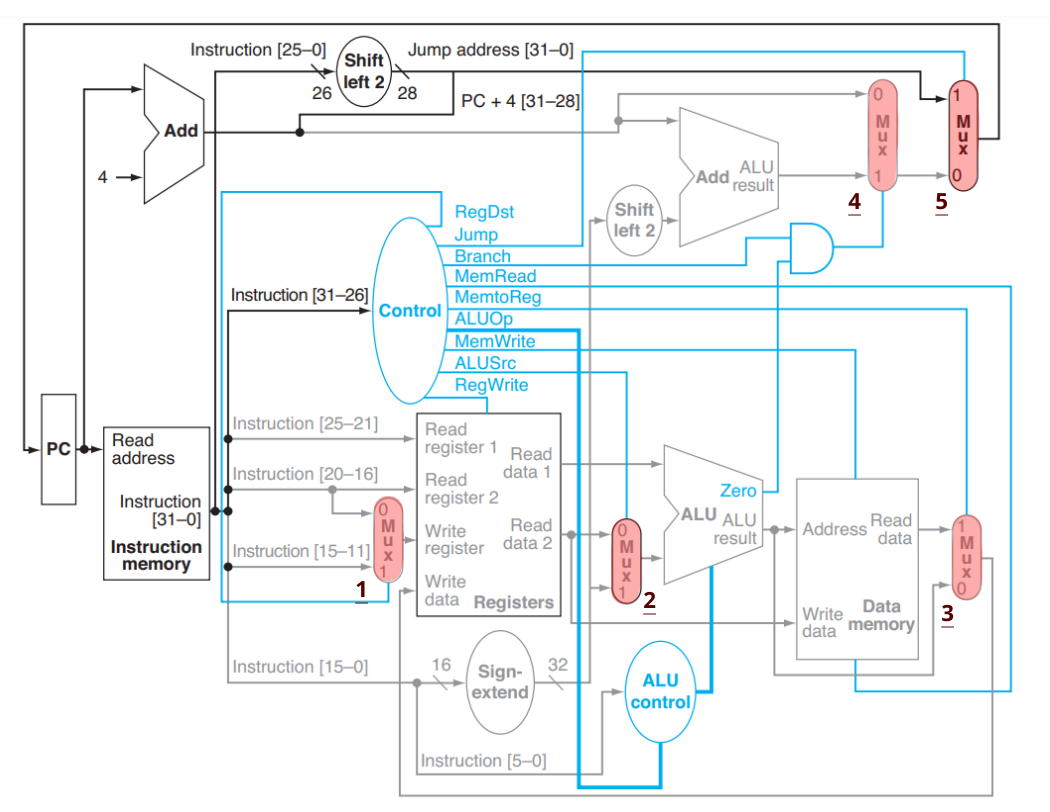
\includegraphics[width=0.7\linewidth]{figs/5.png}$

\setRTL

\begin{enumerate}
	\item 
	چون دستور ما sw است و RegDst برابر صفر است، پس خروجی این مالتیپلکسر برابر است با:
	\setLTR
	
	$MUX_1 = Instruction[20:16]=(00010)_2 = (2)_{10} \rightarrow \$R2$
	
	\setRTL
	
	\item 
	چون سیم مربوط به ALUSrc برابر یک است، پس حاصل واحد Extend Sign مقدار خروجی آن است:
	\setLTR
	
	$MUX_2 = SignExtend(Instruction[15:0])= (14)_{16} = (20)_{10} \rightarrow \$R20$
	
	\setRTL
	
	\item 
	خروجی این مالتیپلکسر برای ما فاقد اهمیت است.
	
	\setLTR
	
	$MUX_3 = \times$
	
	\setRTL
	
	\item 
	سیم مربوط به Branch صفر است، پس خروجی این مالتیپلکسر برابر است با:
	\setLTR
	
	$MUX_4 = PC +4$
	
	\setRTL
	
	\item 
	چون این دستور مربوط به Jump نیست و سیم مربوط به آن صفر است، پس خروجی ما برابر است با:
	\setLTR
	
	$MUX_5 = PC +4$
	
	\setRTL
\end{enumerate}

حال به سراغ دستور b می‌روبم:

\begin{enumerate}
	\item 
	مقدار سیم مربوط به RegDst برابر یک است، پس rd خروجی داده می‌شود:
	\setLTR
	
	$MUX_1 = Instruction[15:11]=(00001)_2 = (1)_{10}$
	
	\setRTL
	
	\item 
	چون سیم مربوط به ALUSrc برابر صفر است، مقدار 2ReadData خروجی داده می‌شود:
	\setLTR
	
	$MUX_2 = Instruction[20:16]= \$rt = \$R2 $
	
	\setRTL	
	
	\item 
	چون سیم مربوط به MemtoReg قطع است، پس خروجی این مالتیپلکسر برابر است با:
	\setLTR
	
	$MUX_3 = ALUResult =slt \ \ \$a_t \ ,\ \$a_0 \ , \ \$v_0 = 0$
	
	\setRTL	
	
	\item 
	بیت کنترلی Branch صفر چون دستور ما مربوط به Branch یا Jump نیست، پس خروجی برابر است با:
	\setLTR
	
	$MUX_4 = PC + 4$
	
	\setRTL	
	
	\item 
	به همان دلیلی که در مورد قبل گفته شد، خروجی برابر است با:
	\setLTR
	
	$MUX_5 = PC + 4$
	
	\setRTL	
\end{enumerate}

\subsubsection*{و}

در این بخش باید ورودی‌های ALU و واحدهای Add موجود در این معماری را محاسبه کنیم. ابتدا به سراغ دستور a می‌رویم:

\begin{enumerate}
	\item ورودی‌های واحد ALU معماری:
	
	\setLTR
	$
	\begin{cases}
		Read1= Instruction[25-21] =\$rs = \$R_3 = (-3)_{10} \\
		Read2 =Instruction[20-16]= address = (20)_{10}
		
	\end{cases}
	$
	\setRTL
	
	\item ورودی‌های واحد Add سمت چپ معماری:
	
	\setLTR
	$
	\begin{cases}
		input1= PC  \\
		input2 = 4
		
	\end{cases}
	$
	
	\setRTL
	
	\item ورودی‌های واحد Add سمت راست معماری:
	
	\setLTR
	
	$
	\begin{cases}
		input1= PC + 4 \\
		input2 = 4 \times Address = 80
		
	\end{cases}
	$
	\setRTL
	
	
\end{enumerate}

\pagebreak

حال به سراغ دستور b می‌رویم:


\begin{enumerate}
	\item ورودی‌های واحد ALU معماری:
	
	\setLTR
	$
	\begin{cases}
		Read1= Instruction[25-21] =\$rs = \$R_2 = -128 \\
		Read2 =Instruction[20-16]= \$rt =\$R_4 = -32
		
	\end{cases}
	$
	\setRTL
	
	\item ورودی‌های واحد Add سمت چپ معماری:
	
	\setLTR
	$
	\begin{cases}
		input1= PC  \\
		input2 = 4
		
	\end{cases}
	$
	
	\setRTL
	
	\item ورودی‌های واحد Add سمت راست معماری:
	
	\setLTR
	$
	\begin{cases}
		input1= PC + 4  \\
		input2 = 4 \times Address = 8360
		
	\end{cases}
	$
	
	\setRTL
	
\end{enumerate}
\pagebreak
\subsubsection*{ز}

در این بخش باید مقادیر مختلف File Register را به ازای هر دو دستور مشخص کنیم. به ازای دستور a مقادیر این ثبات‌ها برابر هستند با:

\setLTR

\begin{itemize}
	\item ReadRegister1 = 3
	\item ReadRegister2 = 2
	\item WriteRegister = 2
	\item WriteData = $\times$
	\item RegWrite = 0
\end{itemize}
\setRTL


حال به سراغ دستور b می‌رویم:

\setLTR

\begin{itemize}
	\item ReadRegister1 = 4
	\item ReadRegister2 = 2
	\item WriteRegister = 1
	\item WriteData = 0
	\item RegWrite = 1
\end{itemize}

\setRTL
